\section*{Conclusion}

Our implementation worked exactly as expected on small and medium size tests, on larger tests, more than 50 processes, the algorithm still elected one process correctly. In those large tests there were some small synchronization problems that can be easily explained by the large number of processes trying to communicate with each other at the same time.

To guarantee that our implementation has the message complexity of the algorithm we the number of messages and the evolution of the $ n log(n)$ function. In Figure \ref{ComplexityAnalysis} you can see clearly that the two lines have the same evolution. The axis are in a logarithmic scale that allows us to represent both functions as almost straight lines.

\begin{figure}[h] \centering
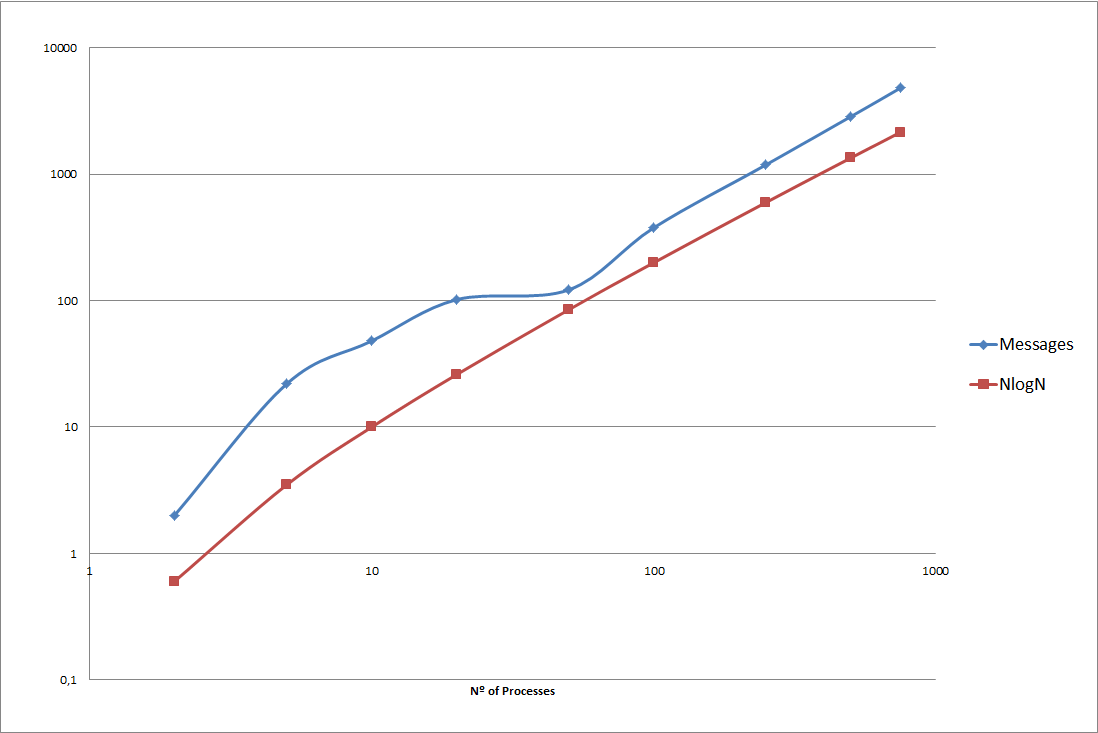
\includegraphics[scale=0.5]{ComplexityAnalysisPlot}\caption{Complexity Analisys of the implementation} \label{ComplexityAnalysis}
\end{figure}
	